\section{Results: research questions}
\label{sec:results}

Table~\ref{tab:answers} gives a short answer to each of the nine questions. This section gives the evidence for the three
research questions, and Section~\ref{sec:eqs} for the six experimental ones. Each subsection starts with the answer, then
gives the evidence and the reasons behind it, and ends with what it means for a researcher.

\begin{table}[t]
\centering
\small
\caption{The questions and their short answers.}
\label{tab:answers}
\begin{tabular}{@{}p{0.27\linewidth}p{0.63\linewidth}l@{}}
\toprule
question & short answer & \S \\
\midrule
RQ1: Does confidence triage coding? & Partly. Ranking quality varies widely across decision models (error AUROC 0.69--0.79;
Sonnet's verbalized confidence 0.80), and how much can be accepted depends mostly on the task. & \ref{sec:rq1} \\
RQ2: Is uncertainty high where humans disagree? & Yes, moderately, for most coders; no coder falls below the range of
individual annotators. & \ref{sec:rq2} \\
RQ3: How stable are decisions? & Mostly stable to rewording, less so to option order; removing context changes 15--24\% of
dialogue labels. & \ref{sec:rq3} \\
\midrule
EQ1: Does calibration error predict triage? & No. Low calibration error does not imply good ranking, and recalibration fixes
calibration without changing ranking. & \ref{sec:eq1} \\
EQ2: Do threshold rules keep their target? & The usual rule overshoots in about half of re-splits. A corpus guarantee holds,
certifying 60--83\% of comment decisions for most coders and none on dialogue at our budgets. & \ref{sec:eq2} \\
EQ3: Ranking or ties at the top? & Both. Large, error-prone ties limit Jev and OpenAI Decisions; per-code maps split ties and
improve ranking for every coder with enough data. & \ref{sec:eq3} \\
EQ4: Do related 9B decision models beat a 9B instruct model? & Against its verbalized confidence, yes; against its token
probabilities, barely. & \ref{sec:eq4} \\
EQ5: What gives the most guaranteed automation per dollar? & pplx-decider per inference dollar; several decision-model
configurations come within two points of Sonnet at a fraction of its cost, but a person still reads most comments. &
\ref{sec:eq5} \\
EQ6: Are the results artefacts? & The checks bound the main threats; the human labels themselves contain errors. &
\ref{sec:eq6} \\
\bottomrule
\end{tabular}
\end{table}

\subsection{RQ1: Does confidence triage qualitative coding?}
\label{sec:rq1}

\textbf{Answer: partly.} Confidence ranks coding errors well above chance for most coders, but how well depends on the coder
more than on the interface, and how much can be accepted depends on the task more than on either.
Table~\ref{tab:main_rq1} summarizes agreement and ranking for every signal, Table~\ref{tab:main_claims} gives the
confirmatory contrasts, and Figures~\ref{fig:forest} and~\ref{fig:rc} show the contrasts and the per-task risk--coverage
curves.

\paragraph{Decision models differ widely in how well they rank their errors.} The open Kev-27B ranks its own errors best among
the decision models (error AUROC 0.788), close to Sonnet's verbalized confidence (0.801). pplx-decider (0.764) and Jev (0.756)
follow; OpenAI Decisions, Clef, Clef-flash and Kev-9B rank errors worse (0.694--0.736). In the pre-specified contrasts, Jev
ranks its errors better than four of the six other decision models: OpenAI Decisions by \res{rq1/jev/oaid/auroc/dci}, Clef by
\res{rq1/jev/clef/auroc/d}, Clef-flash by \res{rq1/jev/clef_flash/auroc/d} and Kev-9B by \res{rq1/jev/kev9b/auroc/d}. Its
difference from pplx-decider is not significant (\res{rq1/jev/pplx/auroc/dci}), though pplx-decider accepts more decisions
under the naive 5\%-target rule (\res{rq1/jev/pplx/cov/dci}). Kev-27B beats Jev on both primary metrics
(\res{rq1/jev/kev27b/auroc/d} AUROC; \res{rq1/jev/kev27b/cov/d} coverage).

\paragraph{Jev beats most LLM confidence signals, but not the strongest verbalized ones.} Jev ranks its errors
better than every token-probability signal, by 0.20 AUROC for Luna and gpt-oss and by 0.07 for the Qwen models, and better than
3-LLM agreement (\res{rq1/jev/agree3/auroc/d}), self-consistency (\res{rq1/jev/luna_sc-vote/auroc/d}) and gpt-oss's verbalized
confidence (\res{rq1/jev/oss-verbal/auroc/d}). The verbalized confidence of Haiku (\res{rq1/jev/haiku-verbal/auroc/d}) and
Sonnet beats it: \res{rq1/jev/sonnet_sub-verbal/auroc/dci} on the pre-specified Sonnet subset
($p=\res{rq1/jev/sonnet_sub-verbal/auroc/p}$) and \res{rq1/jev/sonnet-verbal/auroc/dci} on the full-sample extension. Jev's
advantage over Luna's verbalized confidence is borderline (\res{rq1/jev/luna-verbal/auroc/dci}, bootstrap
$p=\res{rq1/jev/luna-verbal/auroc/p}$) and not a claim after Holm adjustment, and the exploratory Qwen3.8-2.4T's verbalized
confidence edges out Jev (\res{rq1/jev/qwen_big-verbal/auroc/dci}). Token probabilities fail for a simple reason: they
saturate. Read after a generated rationale, 96--100\% of decisions carry confidence $\ge$0.99, so there is almost nothing left
to separate errors from correct labels. What drives the differences among the decision models themselves is the subject of
EQ1, EQ3 and EQ4: calibration, ties at the top of the scale and the read-out.

\paragraph{How much can be accepted depends on the task, and on what is being accepted.} Under the naive rule, Kev-27B, Sonnet
and pplx-decider accept 41--44\% of all decisions and Jev 33\% (Table~\ref{tab:main_policies}; equal-weight means over the five
tasks), but 6.2--7.5\% of what they accept is wrong. Acceptance is far higher on MFRC, where these four accept 78--94\% of
decisions, than on the four dialogue tasks (22--32\% on average). The difference is mostly about what the decisions are. On
MFRC, 89\% of test decisions are codes that do not apply, and most of those are easy: a prevalence baseline that reads no text,
predicting ``absent'' for every code with confidence equal to that code's calibration share of absent labels, accepts 75\% of
MFRC decisions at 3.6\% error under the naive rule (Table~\ref{tab:main_mfrc}), although it carries no certificate
(\S\ref{sec:eq5}). The models differ in what the baseline cannot do, which is to find the codes that apply: among accepted
decisions, pplx-decider labels 62\% of the applying codes correctly, Sonnet 53\% and Jev 35\%, and the rest go to a person or
are missed. Dialogue decisions, by contrast, are choices between neighbouring codes, such as a reflection and a question, and
there the naive rule's error targets mostly fail (\S\ref{sec:eq2}).

\paragraph{Robustness.} Against the adjudicated reference, 39 of the 40 Jev contrasts (20 comparators, two metrics) keep their
sign and significance. The exception is the borderline error-ranking contrast with Luna's verbalized confidence, whose interval
moves from just above zero to just below it (\res{rq1_adj_plan_v1/jev/luna-verbal/auroc/dci}).

\paragraph{What it means.} ``Decision model'' names an interface, not a level of quality: ranking has to be measured on the
researcher's own hand-coded sample, and a strong LLM's verbalized confidence is a competitive alternative. A high accepted
share is not evidence of a useful coder by itself; it should be compared with a baseline that reads nothing and with the
share of applying codes found. And the naive rule's 5\% is a target, not a guarantee: the leading coders' accepted decisions
are wrong 6--7.5\% of the time, which Section~\ref{sec:eq2} explains.

\begin{table}[t]
\centering
\small
\caption{RQ1: agreement, calibration and error ranking on the test split (mean over the five tasks, design-weighted). Groups: decision models, verbalized LLM confidence, token probabilities, agreement signals.}
\label{tab:main_rq1}
\begin{adjustbox}{max width=\linewidth}
\begin{tabular}{llrrrrr}
\toprule
signal & sample & $\kappa$ (weighted) & ECE & error AUROC & AURC & conf $\geq$ 0.99 \\
\midrule
Jev & full & 0.475 & 0.120 & 0.756 & 0.144 & 0.220 \\
OpenAI Decisions & full & 0.449 & 0.122 & 0.736 & 0.155 & 0.309 \\
Clef (27B) & full & 0.377 & 0.055 & 0.721 & 0.228 & 0.000 \\
Clef-flash (9B) & full & 0.369 & 0.065 & 0.712 & 0.234 & 0.000 \\
pplx-decider & full & 0.482 & 0.052 & 0.764 & 0.122 & 0.084 \\
Kev-9B & full & 0.300 & 0.100 & 0.694 & 0.281 & 0.000 \\
Kev-27B & full & 0.474 & 0.073 & 0.788 & 0.105 & 0.003 \\
\midrule
Luna verbal & full & 0.483 & 0.180 & 0.741 & 0.146 & 0.226 \\
Haiku verbal & full & 0.465 & 0.154 & 0.783 & 0.149 & 0.003 \\
gpt-oss verbal & full & 0.452 & 0.204 & 0.727 & 0.192 & 0.043 \\
Qwen3.5-9B verbal & full & 0.383 & 0.303 & 0.646 & 0.276 & 0.389 \\
Sonnet verbal & full & 0.529 & 0.051 & 0.801 & 0.108 & 0.026 \\
Qwen3.8-2.4T verbal & 270/task & 0.499 & 0.102 & 0.802 & 0.122 & 0.002 \\
\midrule
Luna logprob & full & 0.483 & 0.243 & 0.558 & 0.225 & 0.990 \\
gpt-oss logprob & full & 0.452 & 0.284 & 0.558 & 0.264 & 0.998 \\
Qwen3.5-9B logprob & full & 0.384 & 0.334 & 0.684 & 0.237 & 0.964 \\
Qwen3.8-2.4T logprob & 270/task & 0.499 & 0.248 & 0.703 & 0.148 & 0.961 \\
\midrule
3-LLM agreement & full & 0.493 & 0.153 & 0.670 & 0.193 & 0.719 \\
Luna self-consistency & 350/task & 0.506 & 0.196 & 0.624 & 0.197 & 0.851 \\
\bottomrule
\end{tabular}
\end{adjustbox}
\par\smallskip\footnotesize\raggedright Error AUROC: probability that a correct decision is more confident than an incorrect one (ties count half). AURC: area under the risk-coverage curve, lower is better. conf $\geq$ 0.99: share of decisions with confidence $\geq$ 0.99.
\end{table}

\begin{table}[t]
\centering
\small
\caption{Confirmatory contrasts, Jev minus each comparator X, pooled over the five tasks (paired cluster bootstrap, thresholds refitted in every replicate). Positive values favour Jev. Coverage is the naive rule's share accepted.}
\label{tab:main_claims}
\begin{adjustbox}{max width=\linewidth}
\begin{tabular}{llllllll}
\toprule
family & X & \makecell[bl]{$\Delta$ err. AUROC \\{} [95\% CI]} & Holm p & better & \makecell[bl]{$\Delta$ cov@5\% [95\% \\{} CI]} & Holm p & better \\
\midrule
v1.0 & Luna verbal & +0.016 [0.0004, 0.031] & 0.184 & -- & +0.128 [-0.044, 0.180] & 0.510 & -- \\
v1.0 & Haiku verbal & -0.026 [-0.043, -0.011] & 0.016 & X & +0.168 [-0.071, 0.184] & 0.510 & -- \\
v1.0 & gpt-oss verbal & +0.029 [0.011, 0.051] & 0.016 & Jev & +0.108 [-0.064, 0.155] & 0.510 & -- \\
v1.0 & Luna logprob & +0.198 [0.177, 0.221] & 0.016 & Jev & +0.329 [0.148, 0.381] & 0.016 & Jev \\
v1.0 & gpt-oss logprob & +0.198 [0.174, 0.221] & 0.016 & Jev & +0.317 [0.148, 0.367] & 0.016 & Jev \\
v1.0 & 3-LLM agreement & +0.087 [0.069, 0.103] & 0.016 & Jev & +0.329 [0.160, 0.382] & 0.016 & Jev \\
v1.0 & Luna self-consistency & +0.153 [0.118, 0.186] & 0.016 & Jev & +0.164 [0.160, 0.446] & 0.016 & Jev \\
v1.0 & Sonnet verbal (v1.0 subset) & -0.048 [-0.082, -0.015] & 0.016 & X & -0.249 [-0.296, -0.029] & 0.110 & -- \\
\midrule
v1.1 & OpenAI Decisions & +0.020 [0.005, 0.035] & 0.024 & Jev & +0.103 [-0.050, 0.187] & 0.274 & -- \\
\midrule
v1.2 & Clef (27B) & +0.036 [0.017, 0.054] & 0.010 & Jev & +0.090 [-0.085, 0.135] & 1.000 & -- \\
v1.2 & Clef-flash (9B) & +0.045 [0.024, 0.064] & 0.010 & Jev & +0.075 [-0.086, 0.128] & 1.000 & -- \\
v1.2 & pplx-decider & -0.008 [-0.027, 0.010] & 1.000 & -- & -0.079 [-0.245, -0.047] & 0.010 & X \\
v1.2 & Kev-9B & +0.062 [0.041, 0.086] & 0.010 & Jev & +0.090 [-0.041, 0.158] & 0.872 & -- \\
v1.2 & Kev-27B & -0.032 [-0.047, -0.017] & 0.010 & X & -0.113 [-0.272, -0.063] & 0.010 & X \\
\midrule
v1.1 (sec.) & Qwen3.5-9B verbal & +0.110 [0.093, 0.129] & -- & Jev & +0.295 [0.149, 0.364] & -- & Jev \\
v1.1 (sec.) & Qwen3.5-9B logprob & +0.072 [0.050, 0.093] & -- & Jev & +0.236 [0.065, 0.283] & -- & Jev \\
\midrule
ext. & Sonnet verbal (full sample) & -0.045 [-0.060, -0.032] & -- & X & -0.105 [-0.283, -0.055] & -- & X \\
\bottomrule
\end{tabular}
\end{adjustbox}
\par\smallskip\footnotesize\raggedright 'better' names the winner (Jev, or X for the comparator) when the pooled 95\% CI excludes 0 and Holm p < 0.05 within the family; -- : no claim. Holm is part of the plan's rule for v1.2 and a sensitivity analysis for v1.0 and v1.1. Sonnet enters v1.0 as specified, on its nested subset; the full-sample extension (ext.) is exploratory and outside the family. v1.1 secondary rows are unadjusted. Intervals resample each corpus's clusters jointly for related tasks; coverage intervals are asymmetric because refitted thresholds jump between tie blocks.
\end{table}


\begin{figure}[tb]
  \centering
  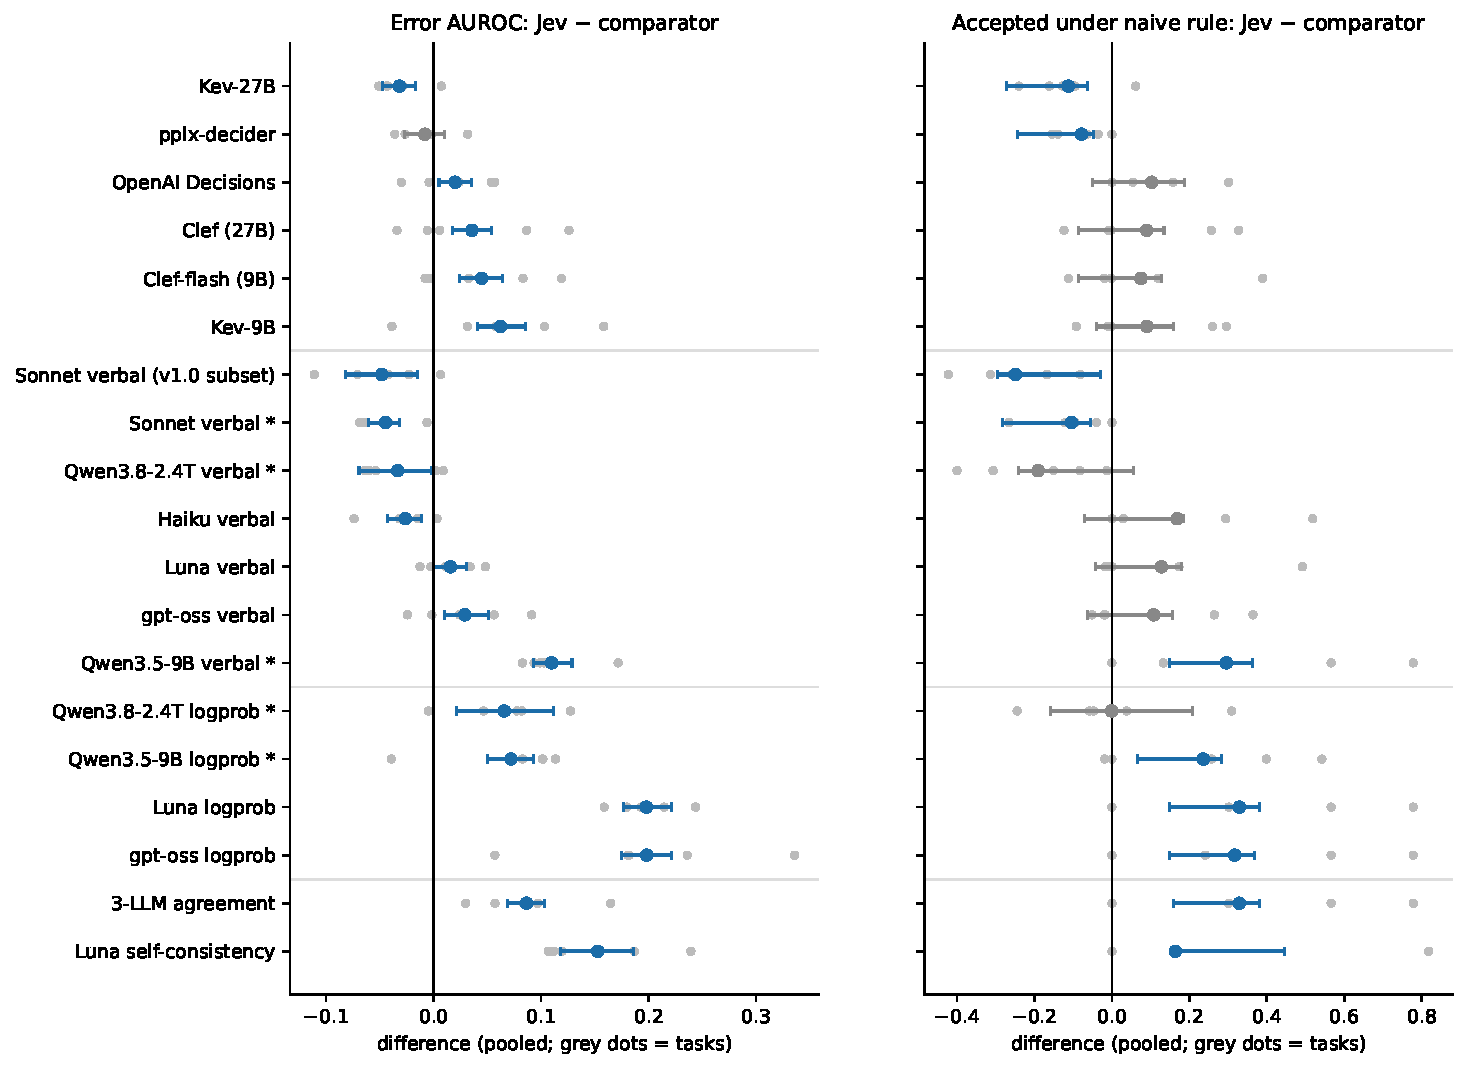
\includegraphics[width=\linewidth]{fig02_forest_jev_contrasts.pdf}
  \caption{RQ1 contrasts: Jev minus each signal, pooled over tasks (grey dots: individual tasks), grouped as decision models,
  verbalized confidence, token probabilities and agreement signals. Positive values favour Jev. Blue marks a 95\% CI that
  excludes 0 (unadjusted). Left: error AUROC. Right: share accepted under the naive 5\%-target rule. *: secondary or
  exploratory comparison (the Qwen models; Sonnet on the full sample, an extension of its pre-specified subset).}
  \label{fig:forest}
\end{figure}

\begin{figure}[tb]
  \centering
  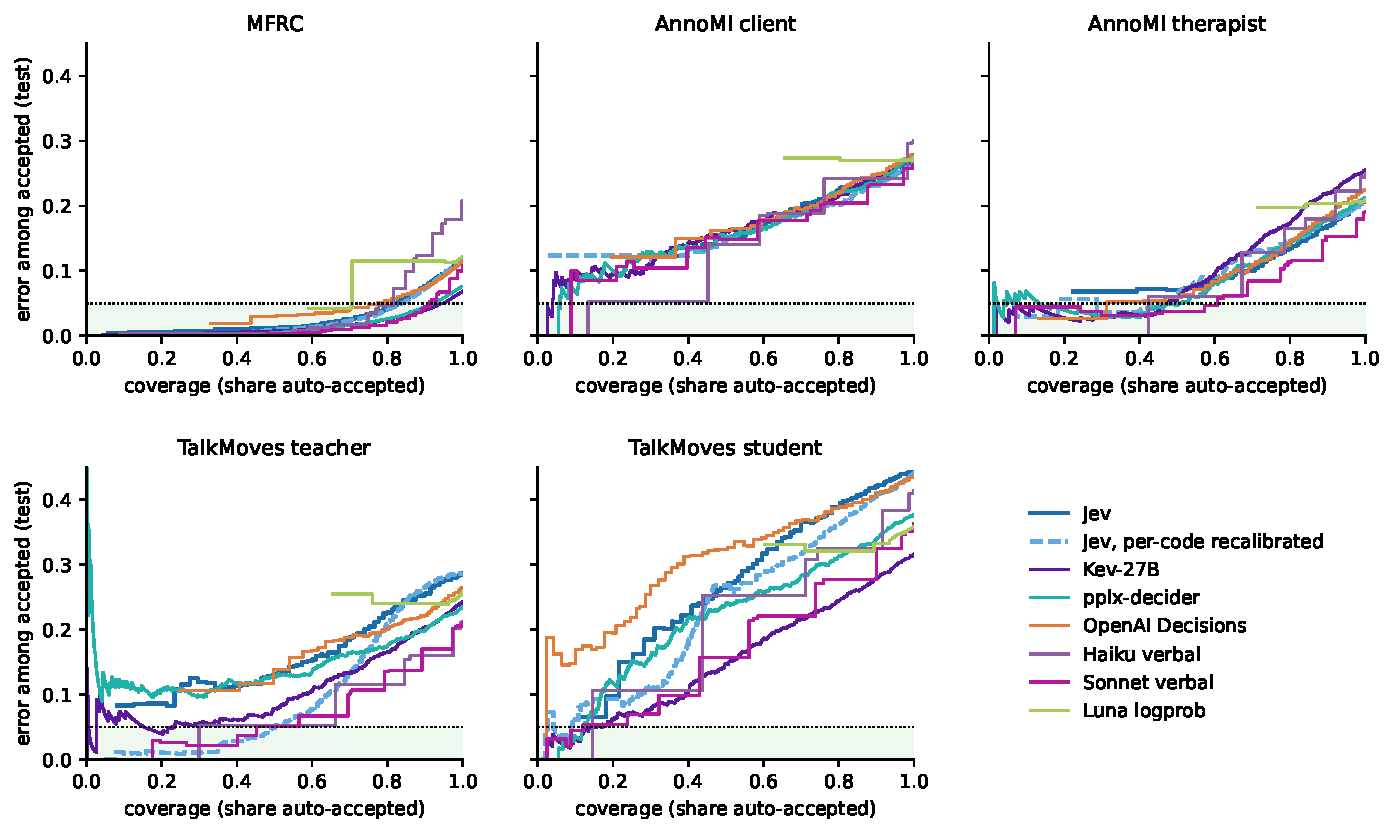
\includegraphics[width=\linewidth]{fig01_risk_coverage.pdf}
  \caption{Risk--coverage on the test split for a subset of coders. Each curve accepts decisions from most to least confident.
  The dotted line is 5\% error, and the shaded band is the region a 5\% target accepts. On the dialogue tasks most coders never
  reach it at any meaningful coverage.}
  \label{fig:rc}
\end{figure}

\begin{table}[t]
\centering
\small
\caption{Threshold policies at a 5\% error target on the frozen split (percent): share of test decisions accepted, and error among them. Pooled columns average the five tasks; dialogue columns average the four dialogue tasks.}
\label{tab:main_policies}
\begin{adjustbox}{max width=\linewidth}
\begin{tabular}{lrrrrrrrrr}
\toprule
signal & \makecell[br]{naive: \\{} accepted} & naive: error & \makecell[br]{oracle: \\{} accepted} & \makecell[br]{MFRC: LTT on \\{} decisions} & \makecell[br]{MFRC: corpus \\{} LTT} & its error & \makecell[br]{dialogue: \\{} naive} & \makecell[br]{dialogue: LTT \\{} on decisions} & \makecell[br]{dialogue: \\{} corpus LTT} \\
\midrule
Jev & 32.9 & \textbf{6.8} & 16.3 & 74.4 & 59.8 & 1.6 & 21.7 & 0.0 & 0.0 \\
OpenAI Decisions & 22.7 & 4.7 & 17.8 & 65.6 & 0.0 & -- & 10.2 & 0.0 & 0.0 \\
Clef (27B) & 24.0 & \textbf{5.8} & 20.3 & 88.4 & 82.3 & 3.0 & 7.4 & 0.0 & 0.0 \\
Clef-flash (9B) & 25.4 & \textbf{7.0} & 20.7 & 86.7 & 77.9 & 2.7 & 9.5 & 0.0 & 0.0 \\
pplx-decider & 40.8 & \textbf{7.5} & 32.1 & 88.5 & 77.1 & 2.3 & 28.0 & 0.0 & 0.0 \\
Kev-9B & 23.9 & \textbf{6.3} & 19.2 & 82.8 & 67.1 & 2.4 & 8.1 & 0.0 & 0.0 \\
Kev-27B & 44.2 & \textbf{7.0} & 37.2 & 91.3 & 76.6 & 2.1 & 31.7 & 10.6 & 0.0 \\
\midrule
Luna verbal & 20.2 & 4.6 & 16.2 & 79.5 & 64.0 & 2.2 & 5.3 & 0.0 & 0.0 \\
Haiku verbal & 16.1 & 3.2 & 16.8 & 74.9 & 65.8 & 1.7 & 1.4 & 0.0 & 0.0 \\
gpt-oss verbal & 22.1 & \textbf{5.6} & 20.6 & 0.0 & 0.0 & -- & 6.9 & 0.0 & 0.0 \\
Sonnet verbal & 43.4 & \textbf{6.2} & 40.1 & 87.5 & 82.7 & 2.5 & 31.7 & 6.1 & 0.0 \\
Qwen3.8-2.4T verbal & 37.9 & 4.3 & 38.0 & 74.8 & 0.0 & -- & 26.8 & 0.0 & 0.0 \\
\bottomrule
\end{tabular}
\end{adjustbox}
\par\smallskip\footnotesize\raggedright Naive: threshold with calibration error $\leq$ 5\% (the pre-specified rule). Oracle: fitted on test, an unattainable upper bound. LTT on decisions treats decisions as independent and is shown only for comparison; corpus LTT certifies the error of the uncoded remainder (Section~\ref{sec:rules}). Bold: naive-rule error above the 5\% target.
\end{table}

\begin{table}[t]
\centering
\small
\caption{MFRC: what the accepted decisions are (percent). 11\% of test decisions are codes that apply. The prevalence baseline reads no text: it predicts 'absent' for every code, with confidence equal to that code's share of 'absent' labels.}
\label{tab:main_mfrc}
\begin{adjustbox}{max width=\linewidth}
\begin{tabular}{lrrrrrrrr}
\toprule
coder & \makecell[br]{naive: \\{} accepted} & naive: error & \makecell[br]{naive: \\{} applying \\{} codes found} & \makecell[br]{corpus LTT: \\{} accepted} & \makecell[br]{corpus LTT: \\{} error} & \makecell[br]{corpus LTT: \\{} share \\{} 'absent'} & \makecell[br]{corpus LTT: \\{} applying \\{} codes found} & \makecell[br]{corpus LTT: \\{} applying \\{} codes \\{} deferred} \\
\midrule
Jev & 77.8 & 3.8 & 34.6 & 59.8 & 1.6 & 96.6 & 17.1 & 75.8 \\
OpenAI Decisions & 72.5 & 4.4 & 12.9 & 0.0 & -- & -- & 0.0 & 100.0 \\
Clef (27B) & 90.2 & 4.9 & 53.8 & 82.3 & 3.0 & 94.6 & 34.9 & 48.2 \\
Clef-flash (9B) & 89.1 & 4.7 & 57.4 & 77.9 & 2.7 & 94.1 & 35.4 & 52.3 \\
pplx-decider & 91.8 & 4.9 & 61.5 & 77.1 & 2.3 & 93.9 & 38.0 & 51.7 \\
Kev-9B & 87.1 & 4.7 & 39.0 & 67.1 & 2.4 & 99.5 & 2.2 & 83.9 \\
Kev-27B & 94.0 & 4.9 & 54.8 & 76.6 & 2.1 & 96.7 & 21.1 & 66.6 \\
Luna verbal & 79.5 & 3.9 & 45.0 & 64.0 & 2.2 & 93.9 & 30.4 & 62.6 \\
Haiku verbal & 74.9 & 3.4 & 30.2 & 65.8 & 1.7 & 96.1 & 21.3 & 70.7 \\
gpt-oss verbal & 83.0 & 4.4 & 39.1 & 0.0 & -- & -- & 0.0 & 100.0 \\
Sonnet verbal & 89.9 & 4.5 & 52.8 & 82.7 & 2.5 & 94.6 & 35.8 & 50.4 \\
\midrule
prevalence baseline & 75.0 & 3.6 & 0.0 & 0.0 & -- & -- & 0.0 & 100.0 \\
\bottomrule
\end{tabular}
\end{adjustbox}
\par\smallskip\footnotesize\raggedright Accepted: share of test decisions; error: among them; share 'absent': accepted decisions that say a code does not apply; applying codes found: applying codes accepted with the right label, over all applying codes; deferred: applying codes left for a person. The baseline's naive scores are fitted on all calibration comments; for corpus LTT they are fitted on half and certified on the other half. Design-weighted.
\end{table}


\FloatBarrier
\subsection{RQ2: Does uncertainty sit where humans disagree?}
\label{sec:rq2}

\textbf{Answer: yes, moderately, for most coders.} When annotators disagree, a single majority label is a weak target
\citep{plank2022problem,baan2022stop}, so we ask whether model uncertainty is high where humans split. The evidence has a
clear limit: MFRC has 1,382 test comments with three annotators, but AnnoMI's multi-annotated test items (91 client and 93
therapist utterances) come from only four transcripts, so the AnnoMI results describe those conversations.

\paragraph{Uncertainty rises where humans split.} For every decision model and the Luna, Haiku, gpt-oss and Sonnet verbal
signals, the Spearman correlation between model uncertainty and the entropy of the human labels is 0.24--0.43 on MFRC and
0.33--0.65 on AnnoMI, except Kev-9B on AnnoMI client (0.18) (Figure~\ref{fig:rq2}). The signals that rank errors poorly also
miss disagreement: token probabilities, vote-based agreement and Qwen3.5-9B's verbalized confidence track it weakly or not at
all, and Luna's token-probability uncertainty is unrelated or inversely related to it ($-$0.10 and $-$0.03 on AnnoMI). This is
consistent with RQ1: confidence that is spread out can register an item's ambiguity, while saturated confidence cannot.
Coders run on a subset (Qwen3.8-2.4T, self-consistency) have only 20--23 multi-annotated AnnoMI items and are not
interpreted.

\paragraph{No coder falls below the range of individual annotators.} In a leave-one-annotator-out comparison, each annotator
in turn is scored against the majority of the other annotators, and each coder is scored against the same references (the dot
is its mean over references). No coder falls below the range of individual annotators, and some fall above it: on AnnoMI
therapist, Jev's mean $\kappa$ (0.891) exceeds all ten annotators' (0.631--0.886), and on MFRC Sonnet exceeds five of six.
This is a descriptive comparison with a broad human range, not a test of equivalence to a typical annotator.

\paragraph{What it means.} Low model confidence is partly a signal of a contested item, not only of a likely model error. A
triage rule that sends low-confidence items to a person therefore sends them, among others, the items where human judgement
matters most. Agreement with annotators, which RQ2 measures, is not the same as interpretive validity, which it does not.

\begin{figure}[tb]
  \centering
  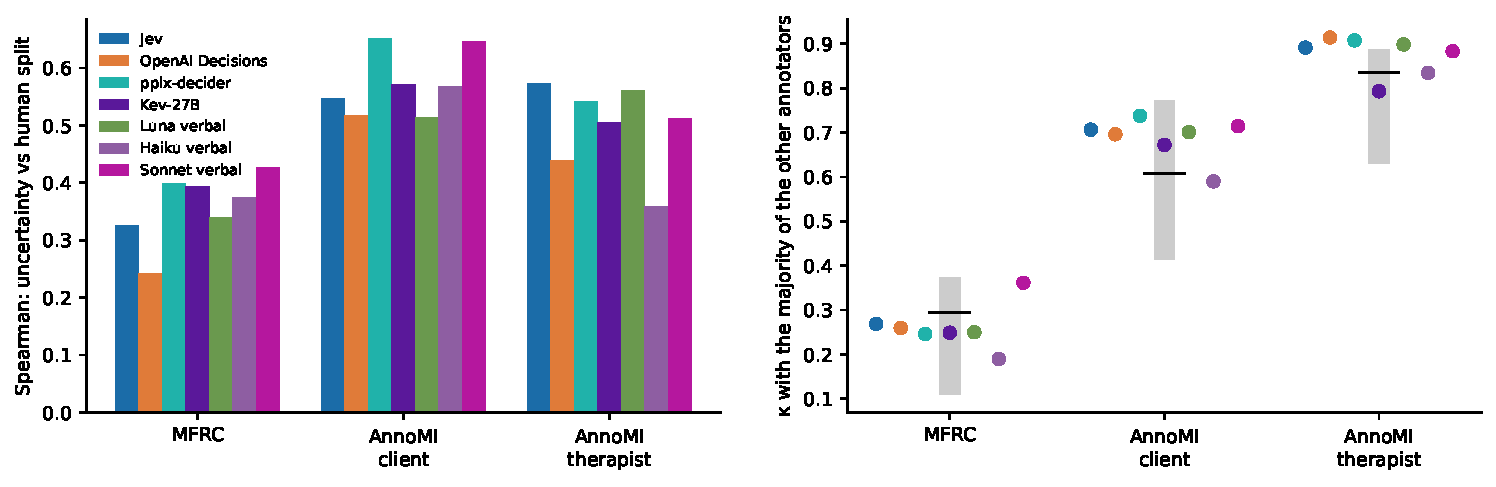
\includegraphics[width=\linewidth]{fig08_rq2_disagreement.pdf}
  \caption{RQ2. Left: Spearman correlation between model uncertainty and human label entropy (MFRC: 1,382 comments; AnnoMI:
  91--93 utterances from four transcripts). Right: $\kappa$ against the majority of the other annotators (grey bar: range over
  individual annotators; tick: median; dots: each model's mean over the same references). Unweighted.}
  \label{fig:rq2}
\end{figure}

\FloatBarrier
\subsection{RQ3: How stable are decisions?}
\label{sec:rq3}

\textbf{Answer: mostly stable to rewording, less so to option order, and dependent on context.} We perturbed the request on
the test split (Figure~\ref{fig:rq3}). Jev, OpenAI Decisions, Clef-flash and pplx-decider ran every arm on all applicable
tasks; Kev-9B ran one to four tasks per arm, because its hosting stopped; Luna and Sonnet ran the option-order and label arms
on 85 test segments per task. Flip rates and changes in AURC, the two pre-specified outcomes, are design-weighted, with
per-task cluster-bootstrap intervals (Table~\ref{tab:tab06_rq3}).
\begin{itemize}
  \item \textbf{Option order matters, differently by model.} Averaged over tasks, reversing or shuffling options changes 4\%
  of Jev's labels, 5--7\% of pplx-decider's and Sonnet's, 8--11\% of OpenAI Decisions' and Luna's, under 1\% of Clef-flash's,
  and 13--31\% of Kev-9B's; in single tasks it reaches 55\% (Kev-9B, reversed options, TalkMoves teacher). For coders whose
  identical repeated requests already vary (2.1\% of Jev's labels, 3.3\% of Sonnet's, 6.6\% of Luna's; \S\ref{sec:eq6}), some
  order flips may reflect that variation; the samples differ, so the rates cannot simply be subtracted.
  \item \textbf{Wording matters a little.} Paraphrased definitions change 3--10\% of labels, and replacing code names with
  neutral identifiers 5--10\%. Asking for MFRC codes one at a time instead of together changes at most 4\% (Clef-flash);
  OpenAI Decisions' multi-label answers are exactly invariant to question order and batching.
  \item \textbf{Removing the previous turn removes information.} It changes 15--24\% of dialogue labels on average over tasks
  (up to 39\% in one task) and makes the coders worse: $\kappa$ falls by 0.012--0.041 and AURC rises by 0.010--0.037. These
  flips are mostly a loss of relevant context, not instability, in line with the finding that added context can redirect
  decision models \citep{xu2026jevout}.
  \item \textbf{Question format has model-specific effects.} Asking each exclusive option as a separate yes/no question
  improves error ranking for Clef-flash ($+$0.029) and pplx-decider ($+$0.022), hurts it for Kev-27B ($-$0.028), and produces no
  clear pooled change for Jev or OpenAI Decisions.
\end{itemize}

\paragraph{Unstable decisions are mostly uncertain ones.} For every coder, the decisions that flip under surface changes are
mostly ones it was already unsure of: a stable decision has higher original confidence than a flipped one with
probability 0.80 (Luna) to 0.96 (Jev), as the median over each coder's task--arm cells. Changes in AURC under surface
perturbations stay within $\pm$0.08 per task for every coder except Kev-9B, whose option-order sensitivity raises AURC by up
to 0.23.

\paragraph{What it means.} Most instability shows up as uncertainty, so triage already sends most unstable decisions to a
person. The exceptions matter in practice: the hand-coded sample and the rest of the corpus should be coded with the same
request, the same option order and the previous turn, and a model with strong position bias, such as Kev-9B, needs its option
order fixed or averaged over; averaging over option rotations \citep{zhang2026anyjev} is a cheap remedy we did not test.

\begin{figure}[tb]
  \centering
  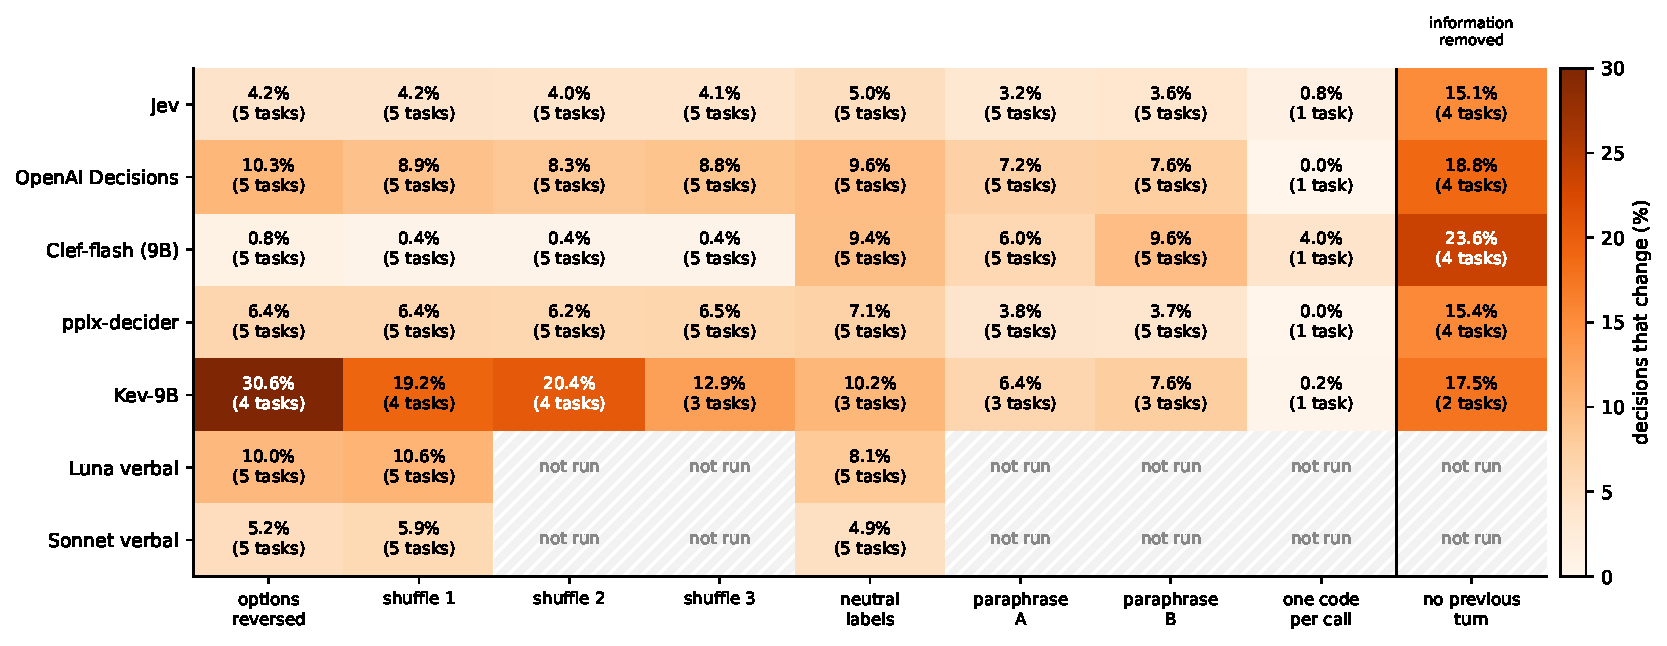
\includegraphics[width=\linewidth]{fig09_rq3_flips.pdf}
  \caption{RQ3: share of decisions that change under each perturbation (design-weighted mean over the tasks each cell
  covers; task counts in brackets). Hatched cells were not run. ``No previous turn'' removes information rather than
  rewording the request.}
  \label{fig:rq3}
\end{figure}
